\documentclass[a4paper,12pt]{article} % добавить leqno в [] для нумерации слева
\usepackage[a4paper,top=1.3cm,bottom=2cm,left=1.5cm,right=1.5cm,marginparwidth=0.75cm]{geometry}
%%% Работа с русским языком
\usepackage{cmap}					% поиск в PDF
\usepackage{mathtext} 				% русские буквы в фомулах
\usepackage[T2A]{fontenc}			% кодировка
\usepackage[utf8]{inputenc}			% кодировка исходного текста
\usepackage[english,russian]{babel}	% локализация и переносы

\usepackage{graphicx}

\usepackage{wrapfig}
\usepackage{tabularx}

\usepackage{hyperref}
\usepackage[rgb]{xcolor}
\hypersetup{
colorlinks=true,urlcolor=blue
}
\usepackage{multirow}
\usepackage{hhline}


%%% Дополнительная работа с математикой
\usepackage{amsmath,amsfonts,amssymb,amsthm,mathtools} % AMS
\usepackage{icomma} % "Умная" запятая: $0,2$ --- число, $0, 2$ --- перечисление

%% Номера формул
\mathtoolsset{showonlyrefs=true} % Показывать номера только у тех формул, на которые есть \eqref{} в тексте.

%% Шрифты
\usepackage{euscript}	 % Шрифт Евклид
\usepackage{mathrsfs} % Красивый матшрифт

%% Свои команды
\DeclareMathOperator{\sgn}{\mathop{sgn}}

%% Перенос знаков в формулах (по Львовскому)
\newcommand*{\hm}[1]{#1\nobreak\discretionary{}
{\hbox{$\mathsurround=0pt #1$}}{}}

\begin{document}
	
	\begin{titlepage}
	\begin{center}
		{\large МОСКОВСКИЙ ФИЗИКО-ТЕХНИЧЕСКИЙ ИНСТИТУТ (НАЦИОНАЛЬНЫЙ ИССЛЕДОВАТЕЛЬСКИЙ УНИВЕРСИТЕТ)}
	\end{center}
	\begin{center}
		{\large Физтех-школа электроники, фотоники и молекулярной физики}
	\end{center}
	
	
	\vspace{4.5cm}
	{\huge
		\begin{center}
			{Лабораторная работа 1.3.3}\\
			Измерение вязкости воздуха по течению в тонких трубках
		\end{center}
	}
	\vspace{2cm}
	\begin{flushright}
		{\LARGE Салтыкова Дарья \\
			\vspace{0.5cm}
			Б04-105}
	\end{flushright}
	\vspace{8cm}
	\begin{center}
		Долгопрудный 2022
	\end{center}
\end{titlepage}

\section{Введение}

\textbf{Цель работы:} экспериментально исследовать свойства течения газов по тонким трубкам при различных числах Рейнольдса; выявить область применимости закона Пуазейля и с его помощью определить коэффициент вязкости воздуха.
\medskip

\noindent \textbf{Оборудование:} система подачи воздуха (компрессор, поводящие трубки); газовый счетчик барабанного типа; спиртовой микроманометр с регулируемым наклоном; набор трубок различного диаметра с выходами для подсоединения микроманометра; секундомер.
\medskip

\section{Теоретические сведения}

\noindent Рассмотрим движение вязкой жидкости или газа по трубке круглого сечения. При малых скоростях потока движение оказывается ламинарным (слоистым), скорости частиц меняются по радиусу и направлены вдоль оси трубки. С увеличением скорости потока движение становится турбулентным, и слои перемешиваются. При турбулентном движении скорость в каждой точке быстро меняет величину и направление, сохраняется только средняя величина скорости.

\medskip

\noindent Характер движения газа (или жидкости) в трубке определяется безразмерным числом Рейнольдса:

\[Re = \dfrac{u a \rho}{\eta} \text{  } \text{  } \text{  }(1)\]

\noindent где $u$ - скорость потока, $a$ - характерный размер системы (размер, на котором существенно меняется скорость течения), $\rho$ - плотность движущейся среды, $\eta$ - вязкость. Это число имеет смысл отношения
кинетической энергии движения элемента объёма жидкости к потерям энергии из-за трения в нём. $Re \sim  K/A_\text{тр} $ В гладких трубах круглого сечения переход от ламинарного движения к турбулентному происходит при $Re \approx 1000$.

\medskip

\noindent При ламинарном течении объем газа $V$, протекающий за время $t$ по трубе длиной $l$, определяется формулой Пуазейля:

\[Q = \dfrac{\pi R^4}{8 l \eta}(P_1 - P_2) \text{  } \text{  } \text{  }(2)\]

\noindent В этой формуле $P_1 - P_2$ - разность давлений в двух выбранных сечениях 1 и 2, расстояние между которыми равно $l$. Велечину $Q$ обычно называют расходом. Формула (2) позволяет определять вязкость газа по его расходу.

\medskip

\noindent Отметим условия, при которых справедлива формула (2). Прежде всего необходимо, чтобы с достаточным запасом выполнялось неравенство $Re < 1000$. Необходимо также, чтобы при течении не происходило существенного изменения удельного объема газа (при выводе формулы удельный объем считался постоянным). Для жидкости это предположение выполняется практически всегда, а для газа - лишь в тех случаях, когда перепад давлений вдоль трубки мал по сравнению с самим давлением. В нашем случае давление газа равно атмосферному ($10^3$ см вод. ст.), а перепад давлений составляет не более 10 см вод. ст., то есть менее $1\%$ от атмосферного. Формула (2) выводится для участков трубки, на которых закон распределения скоростей газа по сечению не меняется при движении вдоль потока.

\medskip


\noindent При втекании газа в трубку из большого резервуара скорости слоев вначале постоянны по всему сечению (рис. 1). По мере продвижения газа по трубке картина распределения скоростей меняется, так как сила трения о стенку тормозит прилежащие к ней слои. Характерное для ламинарного течения параболическое распределение скоростей устанавливается на некотором расстоянии $l_\text{уст}$ от входа в трубку, которое зависит от радиуса трубки $R$ и числа Рейнольдса по формуле

\[l_\text{уст} \approx  0,2 R \cdot Re \text{ } \text{ } \text{ } (3)\]


\medskip

\begin{figure}[h!]
	\center{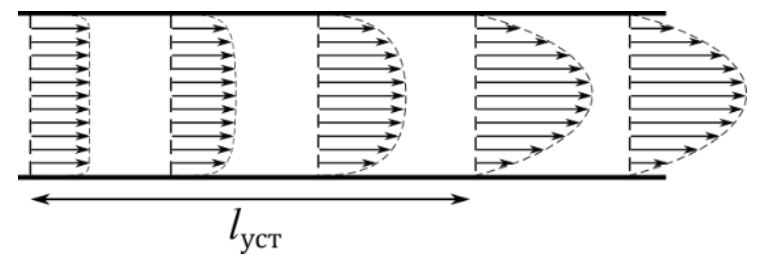
\includegraphics[scale=1]{установление}}
	\caption{Формирование установившегося течения (в ламинарном режиме)}
\end{figure}

\medskip


\noindent Градиент давления на участке формирования потока оказывается большим, чем на участке с установившимся ламинарным течением, что позволяет разделить эти участки экспериментально. Формула (3) дает возможность оценить длину участка формирования.

\medskip

\section{Экспериментальная установка}

\begin{figure}[h]
	\center{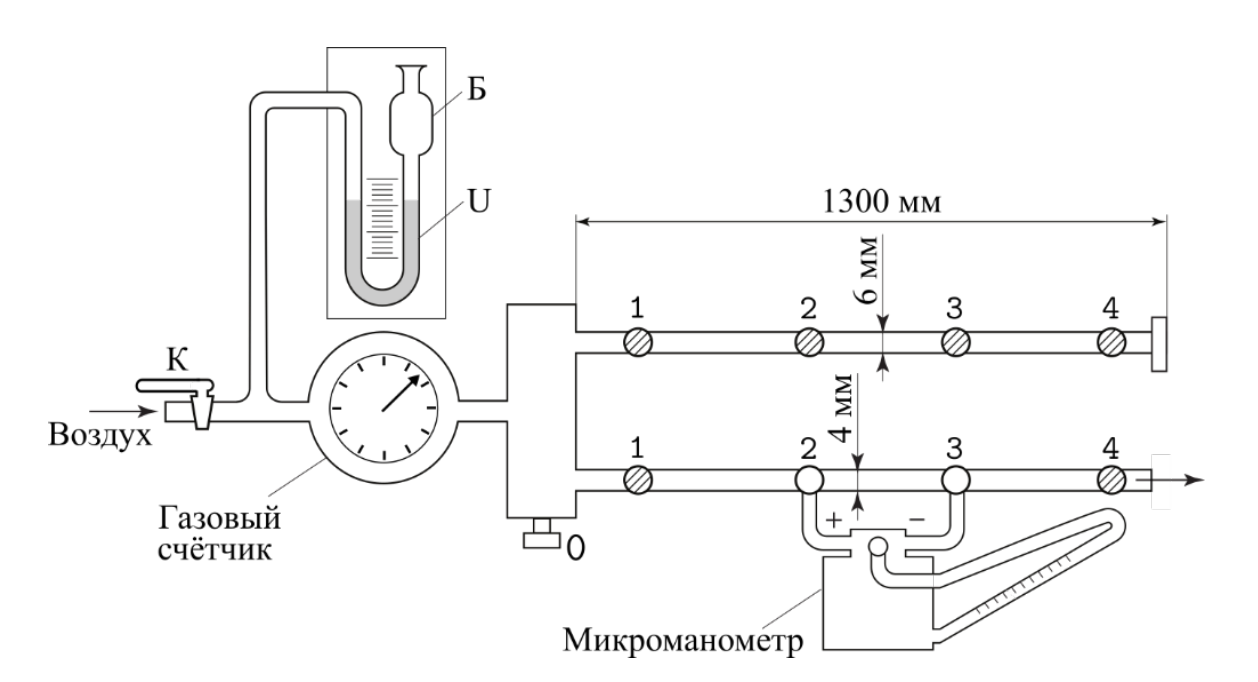
\includegraphics[scale=0.8]{установка}}
	\caption{Экспериментальная установка}
\end{figure}

\medskip

\noindent Схема экспериментальной установки изображена на Рис. 2. Поток воздуха под давлением, немного превышающим атмосферное, поступает через газовый счётчик в тонкие металлические трубки. Воздух нагнетается компрессором, интенсивность его подачи регулируется краном К. Трубки снабжены съёмными заглушками на концах и рядом миллиметровых отверстий, к которым можно подключать микроманометр. В рабочем состоянии открыта заглушка на одной (рабочей) трубке, микроманометр подключён к двум её выводам, а все остальные отверстия плотно закрыты пробками.

\medskip

\noindent Перед входом в газовый счётчик установлен водяной U-образный манометр. Он служит для измерения давления газа на входе, а также предохраняет счётчик от выхода из строя. При превышении максимального избыточного давления на входе счётчика ($\sim 30$ см вод. ст.) вода выплёскивается из трубки в защитный баллон Б, создавая шум и привлекая к себе внимание экспериментатора.

\medskip

\section{Ход работы}

\medskip

\noindent 1. Проведем предварительные расчеты:

\medskip

\noindent 1.1 Рассчитаем значение расхода $Q_\text{кр} $, при котором число Рейнольдса станет равным критическому $ Re_\text{кр} \approx 10^3 $. Для предварительной оценки примем вязкость воздуха равной $\eta_\text{возд} \sim 2 \cdot 10^{-5} \text{Па·с} $, плотность воздуха определим по уравнению идеального газа. В качестве характерной скорости потока используем её среднее значение $\langle u \rangle = \frac{Q}{\pi R^2} $.
	
	$$ Q_\text{кр} = \langle u \rangle \pi R^2 = \frac{Re_\text{кр} \eta_\text{возд} \pi R^2}{\rho l} $$
	
\medskip
	
\noindent Для $d = 3,90 \pm 0,05 \text{ мм}$ $$Q_\text{кр} = 4 \cdot 10^{-7} \text{ м3/с.}$$

\medskip

\noindent Для $d = 5,25 \pm 0,05 \text{ мм}$ $$Q_\text{кр} = 7 \cdot 10^{-7} \text{ м3/с.}$$

\medskip

\noindent Для $d = 3,00 \pm 0,1 \text{ мм}$ $$Q_\text{кр} = 2 \cdot 10^{-7} \text{ м3/с.}$$

\medskip
	
\noindent 1.2  По формуле Пуазейля рассчитаем соответствующий перепад давления на выбранном участке $ \Delta P_\text{кр} $. 
	
\medskip
	
	$$ \Delta P_\text{кр} = \frac{8 \eta l Q}{\pi R^4}$$
	
\medskip
	
\noindent Для $d = 3,90 \pm 0,05 \text{ мм}$ $$\Delta P_\text{кр} = 260 \text{ Па.}$$

\medskip

\noindent Для $d = 5,25 \pm 0,05 \text{ мм}$ $$\Delta P_\text{кр} = 310 \text{ Па.}$$

\medskip	
	
\noindent Для $d = 3,00 \pm 0,1 \text{ мм}$ $$\Delta P_\text{кр} = 200 \text{ Па.}$$

\medskip		
	
\noindent 1.3  Оценим длину $ l_\text{уст} $, на которой течение можно считать установившимся при $ Re \approx Re_\text{кр} $.

\medskip 
	
\noindent Для $d = 3,90 \pm 0,05 \text{ мм}$: $$l_\text{уст} = 39 \text{ см.}$$

\medskip

\noindent Для $d = 5,25 \pm 0,05 \text{ мм}$: $$l_\text{уст} = 52,5 \text{ см.}$$

\medskip	

\noindent Для $d = 5,25 \pm 0,05 \text{ мм}$: $$l_\text{уст} = 30 \text{ см.}$$

\medskip	


\noindent 2. Меняя расход воздуха краном К и наблюдая за столбиком спирта в микроманометре, визуально определим границу перехода $ \Delta P_\text{кр} $ от ламинарного течения к турбулентному (турбулентный режим характеризуется заметными пульсациями давления во времени).

\medskip

\noindent Для $d = 3,90 \pm 0,05 \text{ мм}$: $\Delta P_\text{кр} \approx 224 \text{ Па.}$

\medskip

\noindent Для $d = 5,25 \pm 0,05 \text{ мм}$: $\Delta P_\text{кр} \approx 250 \text{ Па.}$

\medskip

\noindent Для $d = 3,00 \pm 0,1 \text{ мм}$: $\Delta P_\text{кр} \approx 187 \text{ Па.}$

\medskip

\noindent Экспериментальные значения близки к полученным теоретически.

\medskip

\noindent 3. Оценим погрешность измерения времени $\sigma_t$. Для этого проведем серию из 7–9 измерений времени прохождения через счётчик постоянного объёма газа при постоянном расходе и в качестве оценки для случайной погрешности измерения времени используем среднеквадратичное отклонение результатов.

\medskip
\medskip

\begin{tabular}{|c|c|c|c|c|c|c|c|c|}
\hline 
№ & 1 & 2 & 3 & 4 & 5 & 6 & 7 & 8 \\ 
\hline 
$t, \text{с}$ & 12,40 & 12,56 & 12,14 & 11,89 & 12,24 & 12,23 & 12,68 & 12,07 \\ 
\hline 
$\sigma_t, \text{с}$ & \multicolumn{8}{c|}{0,092} \\ 
\hline 
\end{tabular} 

\medskip

\medskip

\noindent 4. Измерим зависимости перепада давления $ \Delta P $ на выбранных участках трубок от расхода газа $Q$.

\medskip

\noindent Для $l = 50 \text{ см}, d = 3,90 \pm 0,05 \text{ мм}$.

\medskip
\medskip

\begin{tabular}{|c|c|c|c|c|c|c|c|c|}
\hline 
$Q, \text{ л/с}$ & 0,032 & 0,072 & 0,089 & 0,095 & 0,109 & 0,119 & 0,128 & 0,134 \\ 
\hline 
$\Delta P, \text{ Па}$ & 49,033 & 121,6 & 168,7 & 200,1 & 276,5 & 339,3 & 396,2 & 429,5 \\ 
\hline 
$\sigma_Q, \text{ л/с}$ & \multicolumn{8}{c|}{0,0028
} \\ 
\hline 
$\sigma_P, \text{ Па}$ & \multicolumn{8}{c|}{5,88} \\ 
\hline 
\end{tabular} 

\medskip
\medskip

\noindent Для $l = 50 \text{ см}, d = 5,25 \pm 0,05 \text{ мм}$.

\medskip
\medskip

\begin{tabular}{|c|c|c|c|c|c|c|c|c|}
\hline 
$Q, \text{ л/с}$ & 0,095 & 0,127 & 0,146 & 0,165 & 0,183 & 0,210 & 0,233 & 0,264 \\ 
\hline 
$\Delta P, \text{ Па}$ & 45,111 & 62,76 & 113,8 & 149,1 & 180,4 & 227,5 & 282,4 & 362,8 \\ 
\hline 
$\sigma_Q, \text{ л/с}$ & \multicolumn{8}{c|}{0,0028
} \\ 
\hline 
$\sigma_P, \text{ Па}$ & \multicolumn{8}{c|}{5,88} \\ 
\hline 
\end{tabular} 

\medskip
\medskip

\noindent Построим графики зависимости $Q(\Delta P)$ (см. Рис. 3 и 4).

\medskip
\medskip

\noindent Из графиков видно, что для $d = 3,90 \pm 0,05 \text{ мм}$: $\Delta P_\text{кр} \approx 190 \text{Па}$; для $d = 5,25 \pm 0,05 \text{ мм}$: $\Delta P_\text{кр} \approx 230 \text{ Па}$.

\medskip
\medskip

\noindent Пользуясь формулой Пуазейля, по угловым коэффициентам линейных участков определим вязкость воздуха $ \eta $. 
$$ \eta = (2,2 \pm 0,4) \cdot 10^{-5} \text{ Па} \cdot \text{с}$$
$$ \eta = (1,3 \pm 0,56) \cdot 10^{-5} \text{ Па} \cdot \text{с}$$

\medskip

\noindent Рассчитаем критическое число Рейнольдса $ Re_\text{кр} $: $ Re_\text{кр} \approx 1950$ (для $d = 3,90 \pm 0,05 \text{ мм}$)

\medskip

\noindent 5. Измерим распределение давления газа вдоль трубки $P(x)$.

\medskip

\noindent Для $Q = 0,128 \text{ л/с}, d = 5,25 \pm 0,05 \text{ мм}$.

\medskip
\medskip

\begin{tabular}{|c|c|c|c|c|}
\hline 
$ \Delta P, \text{ Па}$ & 86,29 & 133,4 & 200,1 & 276,5 \\ 
\hline 
$\sigma_P, \text{ Па}$ & \multicolumn{4}{c|}{5,88}\\
\hline
$ l, \text{ см}$ & 10,5 & 40,5 & 80,5 & 130,5 \\ 
\hline 
$\sigma_l, \text{ см}$ & \multicolumn{4}{c|}{0,5}\\
\hline
\end{tabular} 

\medskip
\medskip

\noindent Для $Q = 0,067 \text{ л/с}, d = 3,90 \pm 0,05 \text{ мм}$.

\medskip
\medskip

\begin{tabular}{|c|c|c|c|c|}
\hline 
$ \Delta P, \text{ Па}$ & 94,1 & 158 & 247 & 359 \\ 
\hline 
$\sigma_P, \text{ Па}$ & \multicolumn{4}{c|}{5,88}\\
\hline
$ l, \text{ см}$ & 11 & 41 & 81 & 131 \\ 
\hline 
$\sigma_l, \text{ см}$ & \multicolumn{4}{c|}{0,5}\\
\hline
\end{tabular} 

\medskip
\medskip

\noindent Для $Q = 0,089 \text{ л/с}, d = 3,00 \pm 0,10 \text{ мм}$.

\medskip
\medskip

\begin{tabular}{|c|c|c|c|}
\hline 
$ \Delta P, \cdot \text{ Па}$ & 100 & 224 & 308  \\ 
\hline 
$\sigma_P, \text{ Па}$ & \multicolumn{3}{c|}{5,88}\\
\hline
$ l, \text{ см}$ & 6 & 26 & 46 \\ 
\hline 
$\sigma_l, \text{ см}$ & \multicolumn{3}{c|}{0,5}\\
\hline
\end{tabular} 

\medskip
\medskip

\noindent По результатам измерений построим графики $P(x)$ зависимостей давления $P$ от координаты вдоль трубы $x$. (cм. Рис. 5)

\medskip

\noindent Из графика оценим длину участка, на котором происходит установление потока:

\medskip

\noindent Для $d = 3,90 \pm 0,05 \text{ мм}: l_\text{уст} \approx 39 \text{см}$

\medskip

\noindent Для $d = 5,25 \pm 0,05 \text{ мм}: l_\text{уст} \approx 38 \text{см}$

\medskip

\noindent Для $d = 3,00 \pm 0,1 \text{ мм}: l_\text{уст} \approx 26 \text{см}$

\medskip

\noindent 6. Измерим зависимость расхода от радиуса трубы при заданном градиенте
давления.

\medskip

\noindent Сначала проведем измерения в ламинарном режиме. Установим $\frac{\Delta P}{l} = \frac{51}{50} \approx 1 \text{ }\frac{\text{мм вод ст}}{\text{см}} = \text{const}$

\medskip

\noindent Для $d = 3,90 \pm 0,05 \text{ мм}, Q = 0,060 \text{ л/с}$.

\medskip
\medskip

\noindent Для $d = 5,25 \pm 0,05 \text{ мм}, Q = 0,20 \text{ л/с}$.

\medskip
\medskip

\noindent Для $d = 3,00 \pm 0,1 \text{ мм}, Q = 0,018 \text{ л/с}$.

\medskip
\medskip

\noindent Теперь проведем измерения в турбулентном режиме. Установим $\frac{\Delta P}{l} = \frac{154}{50} \approx 3 \text{ }\frac{\text{мм вод ст}}{\text{см}} = \text{const}$. 

\medskip
\medskip

\noindent Для $d = 3,90 \pm 0,05 \text{ мм}, Q = 0,111 \text{ л/с}$.

\medskip
\medskip

\noindent Для $d = 5,25 \pm 0,05 \text{ мм}, Q = 0,271 \text{ л/с}$.

\medskip
\medskip

\noindent Для $d = 3,00 \pm 0,1 \text{ мм}, Q = 0,052 \text{ л/с}$.

\medskip
\medskip

\noindent Изобразим результаты на графике в двойном логарифмическом масштабе $lnQ (ln R)$ (Рис. 6). Наклон полученной прямой соответствует показателю степени $ \beta $ зависимости $ Q \sim R^{\beta} $.

\medskip
\medskip

\noindent Для ламинарного режима:
$$ \beta = 4,29 \pm 0,15 $$
\noindent Для турбулентного режима:
$$ \beta = 2,94 \pm 0,03 $$

\medskip
\medskip

\section{Вывод}


\noindent В ходе работы:
	
\begin{itemize}
	\item Были исследованы условия перехода течения из ламинарного режима в турбулентный. 
	
	
	\item Было определено значение вязкости воздуха с помощью трубок разного диаметра: $ \eta = (2,2 \pm 0,4) \cdot 10^{-5} \text{ Па} \cdot \text{с}$;
$ \eta = (1,3 \pm 0,56) \cdot 10^{-5} \text{ Па} \cdot \text{с}$, табличное значение составляет $\eta_{\text{табл}} = 1,78 \cdot 10^{-5}$ Па$\cdot$с. Полученные значения равны в пределах погрешности. Основной вклад в погрешность итогового значения вязкости внесла погрешность измерения давлений.
	
	\item Были получены достаточно близкие к теоретическим значения длин установления для трубок трех диаметров.
	
	\medskip
	
	\noindent Для $d = 3,90 \pm 0,05 \text{ мм}: l_\text{уст} \approx 39 \text{см}$

\medskip

\noindent Для $d = 5,25 \pm 0,05 \text{ мм}: l_\text{уст} \approx 38 \text{см}$

\medskip

\noindent Для $d = 3,00 \pm 0,1 \text{ мм}: l_\text{уст} \approx 26 \text{см}$

	
	\item Было установлено, что расход в ламинарном режиме пропорционален радиусу трубы в $\beta = 4,29 \pm 0,15 $ степени, а в турбулентном режиме - в $ \beta = 2,94 \pm 0,03 $ степени.

\end{itemize}

\noindent Исследуемые зависимости представлены на графиках ниже.
	

\begin{figure}[h!]
\begin{center}
\begin{minipage}[h]{0.45\linewidth}
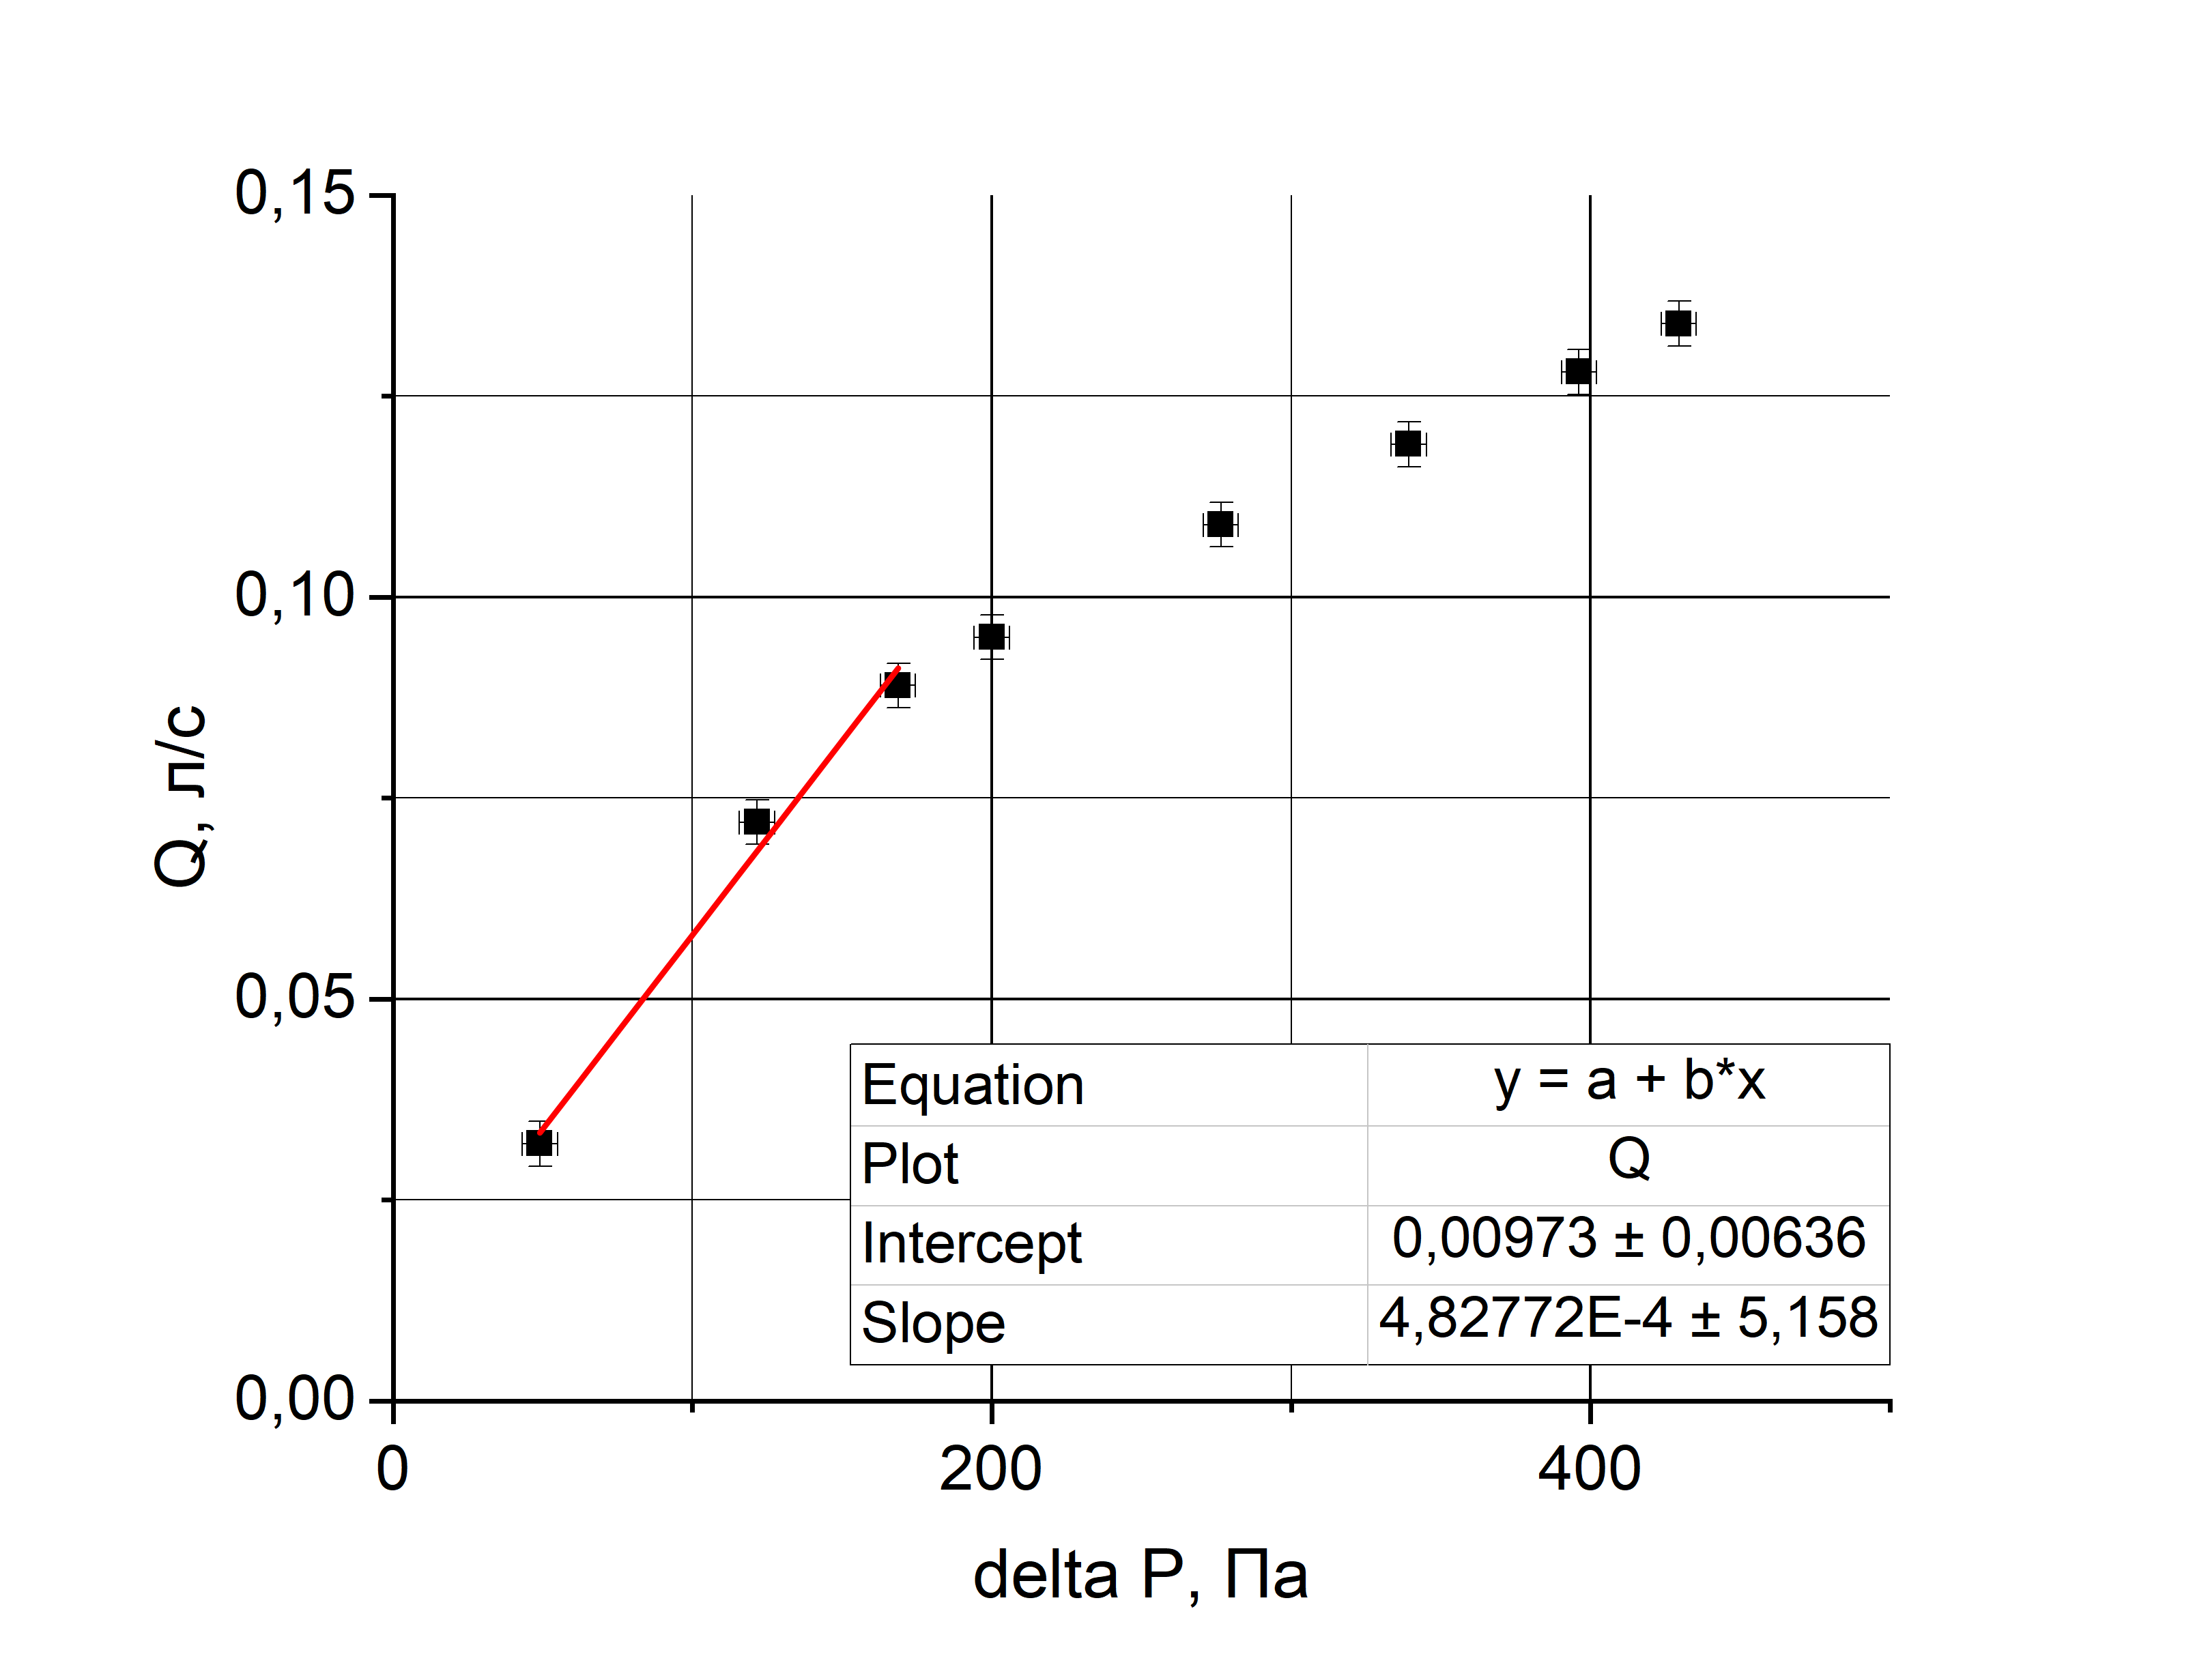
\includegraphics[width=1.2\linewidth]{1d1}
\caption{$d = 3,90 \pm 0,05 \text{ мм}$.} %% подпись к рисунку
\label{ris:experimoriginal} %% метка рисунка для ссылки на него
\end{minipage}
\hfill
\begin{minipage}[h]{0.45\linewidth}
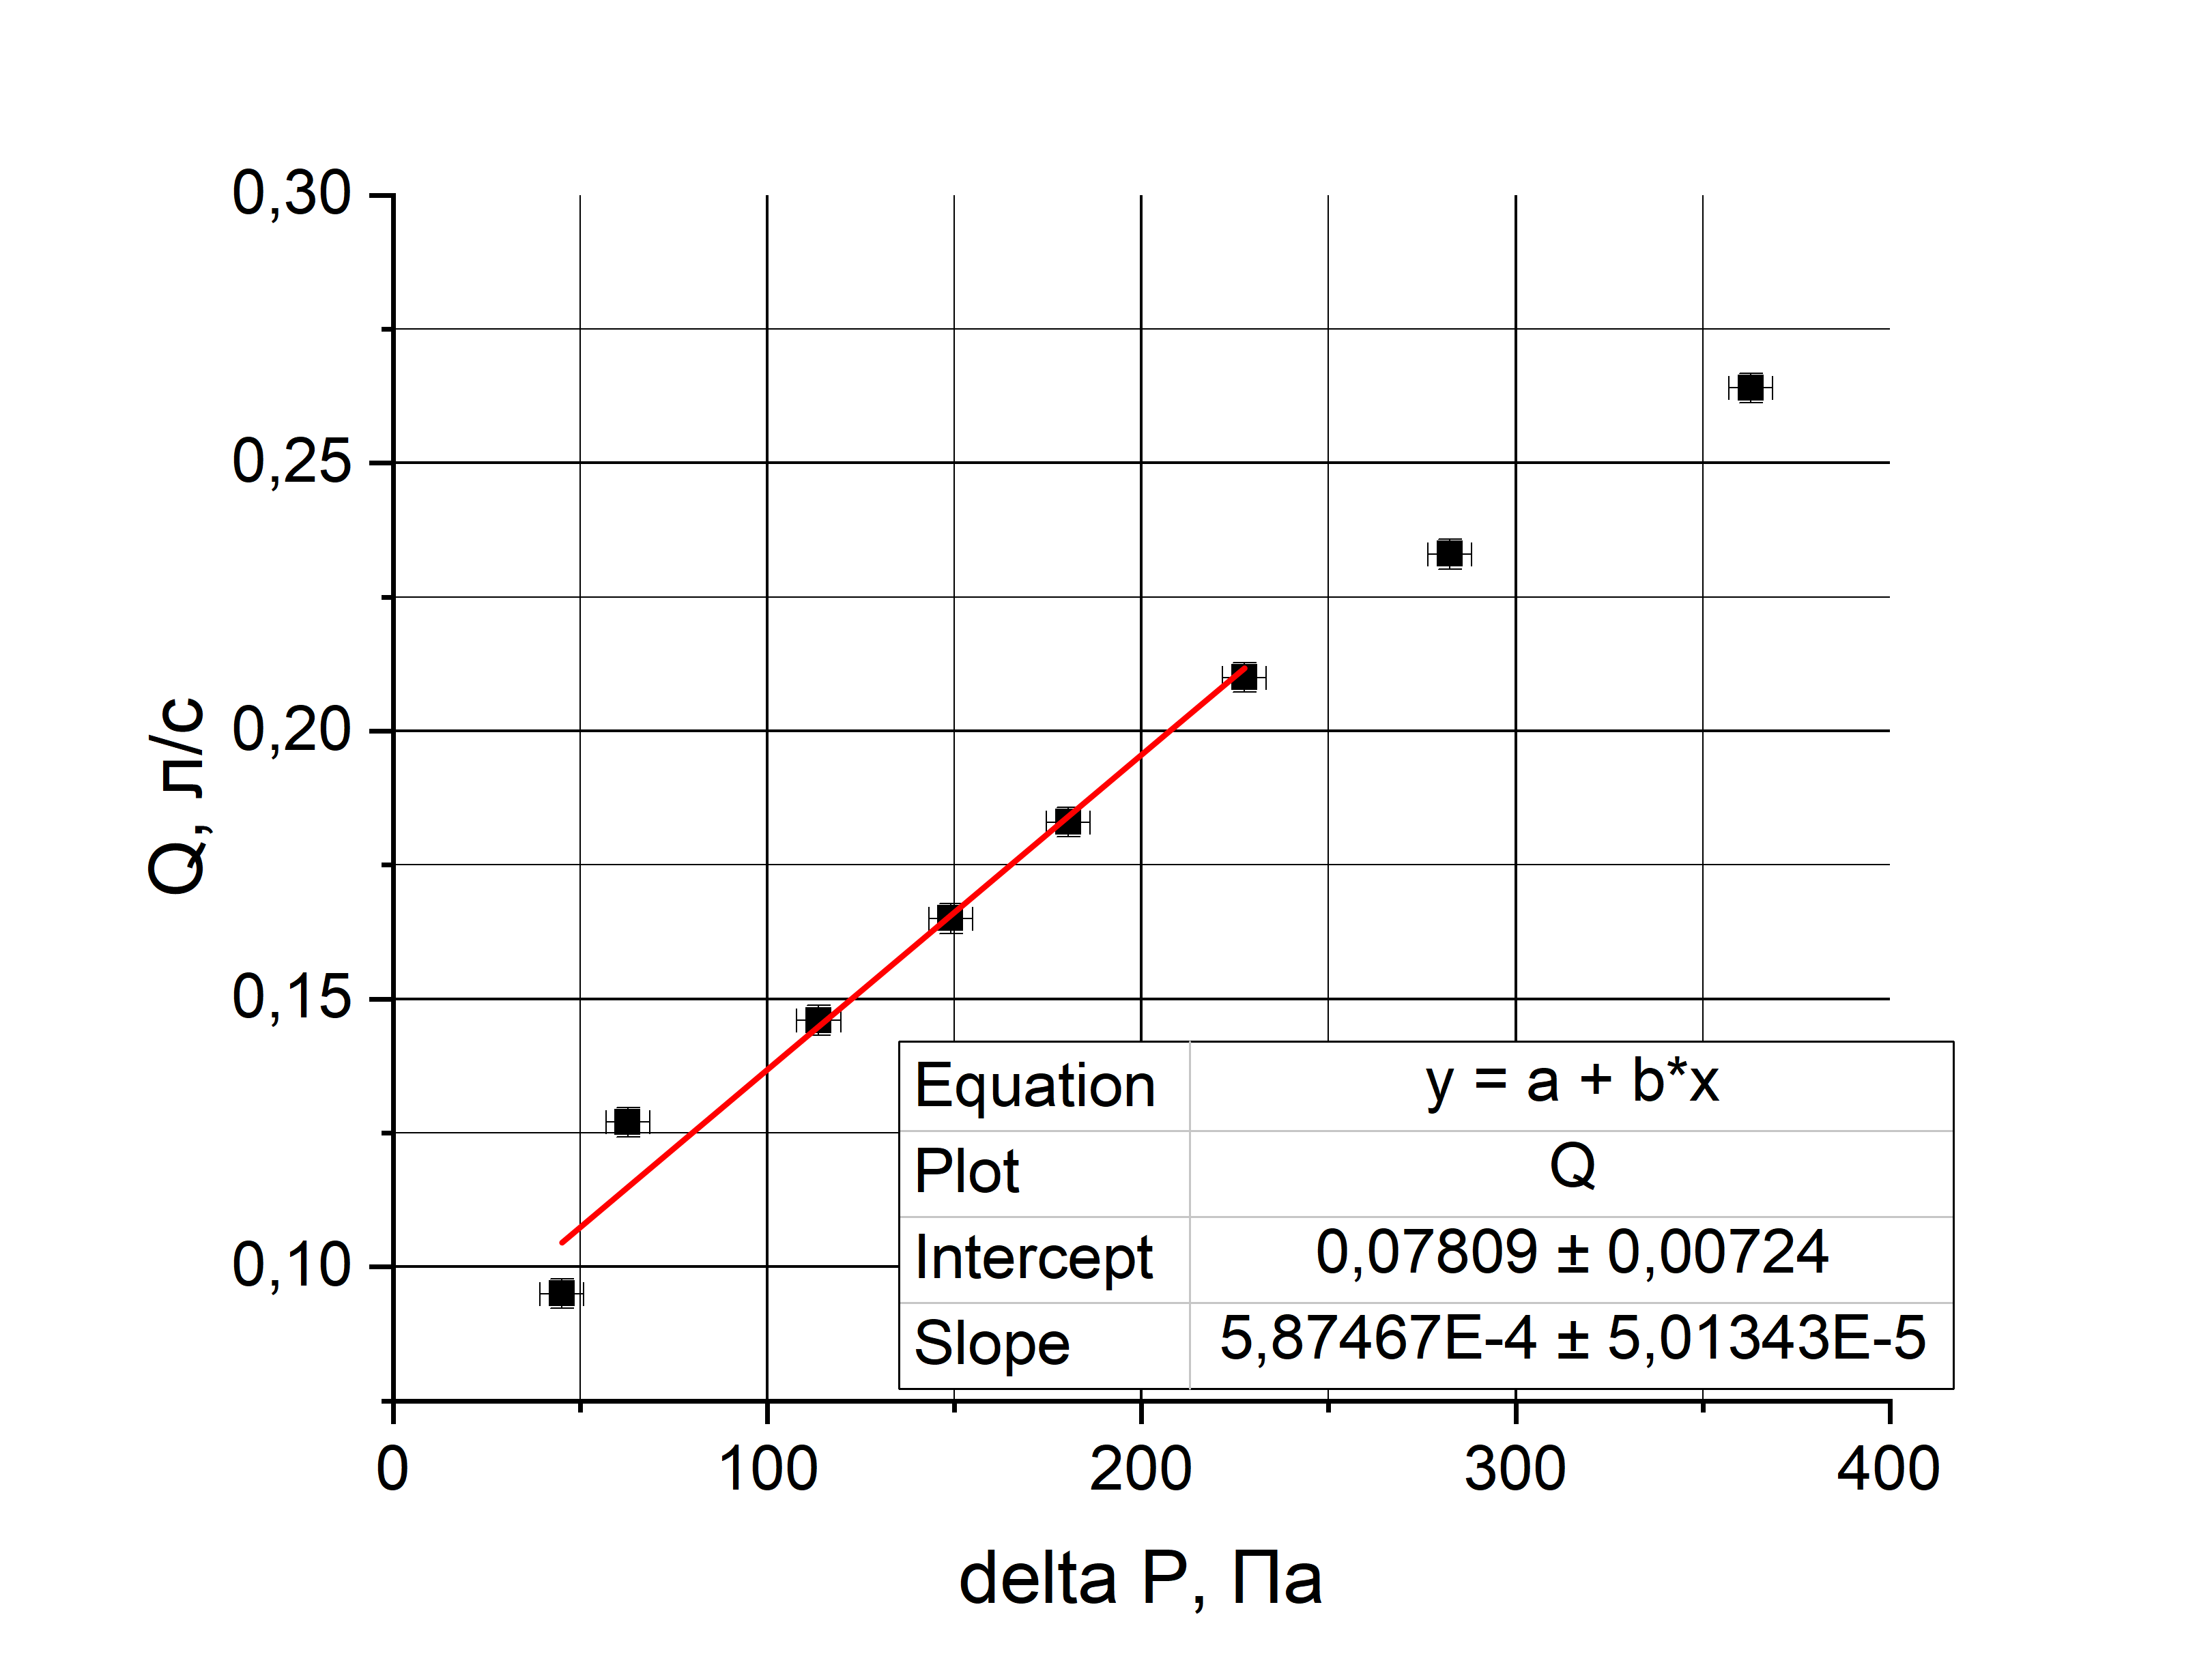
\includegraphics[width=1.2\linewidth]{1d2}
\caption{$d = 5,25 \pm 0,05 \text{ мм}$.}
\end{minipage}
\end{center}
\end{figure}


\begin{figure}[h]
\center{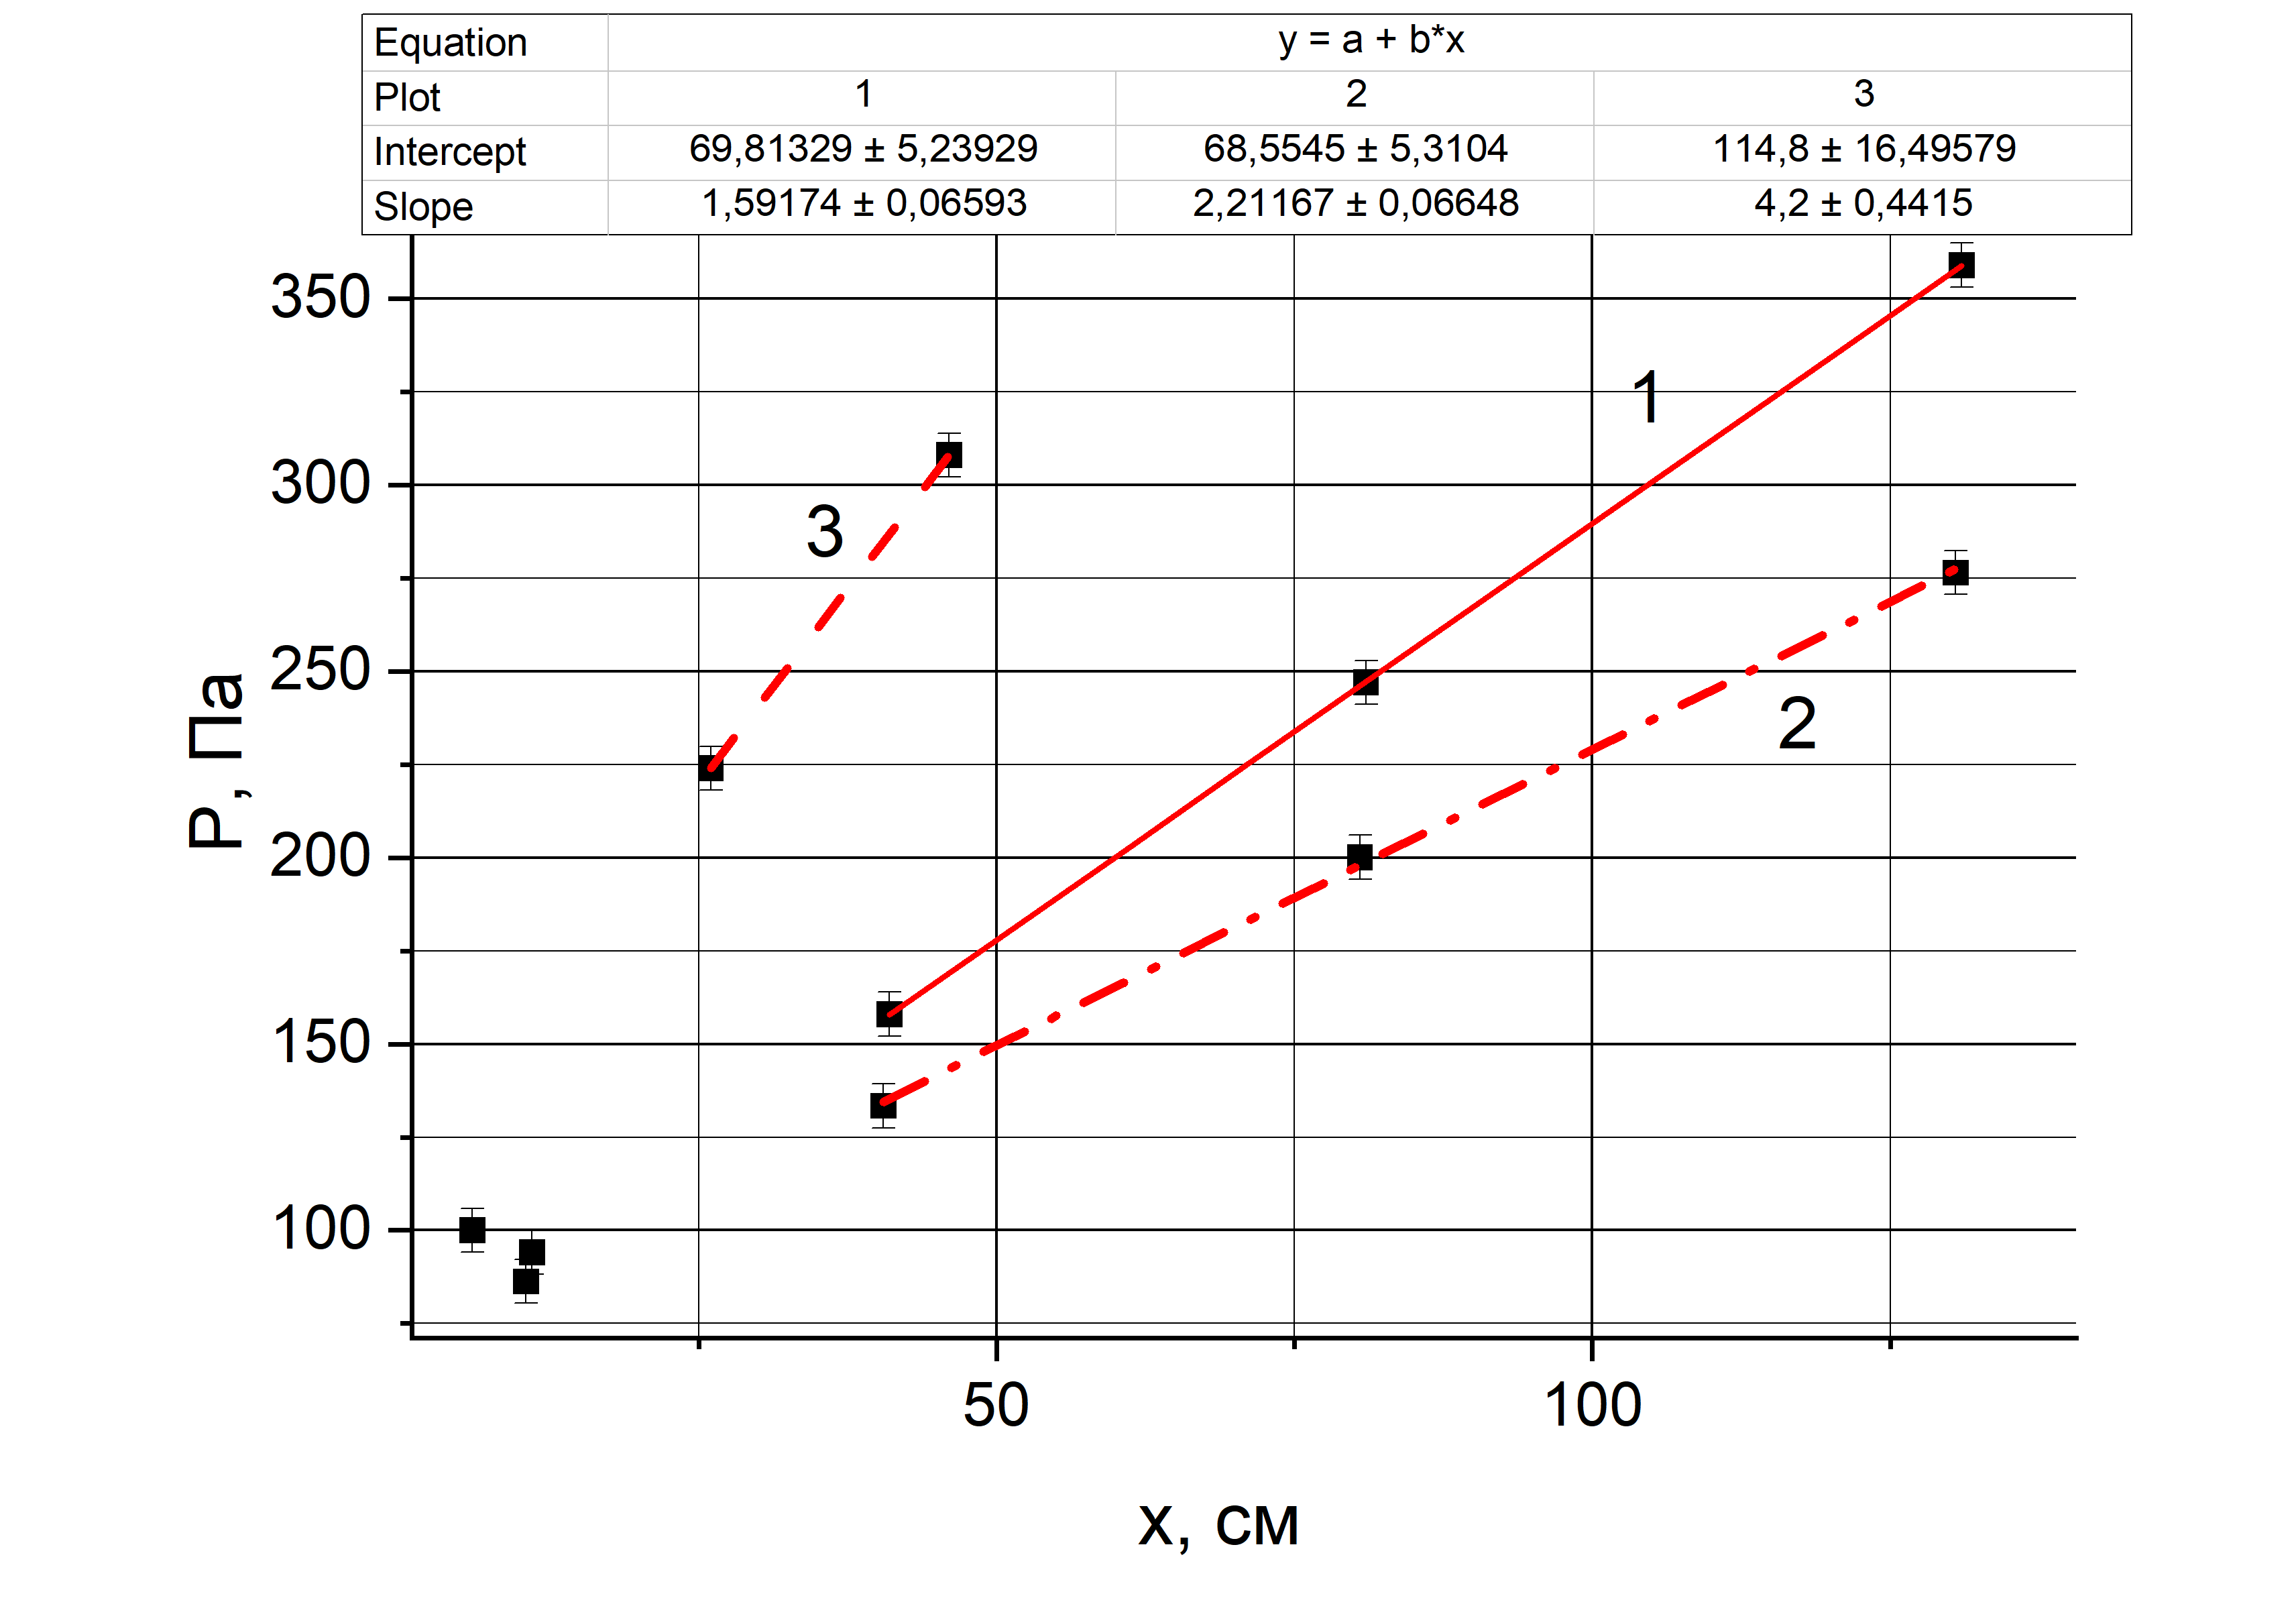
\includegraphics[width=0.7\linewidth]{2}}
\caption{1) $d = 5,25 \pm 0,05 \text{ мм; }$ 2) $d = 3,90 \pm 0,05 \text{ мм; }$\\ 3) $d = 3,00 \pm 0,10 \text{ мм}$.}
\end{figure}

\begin{figure}[h!]
\center{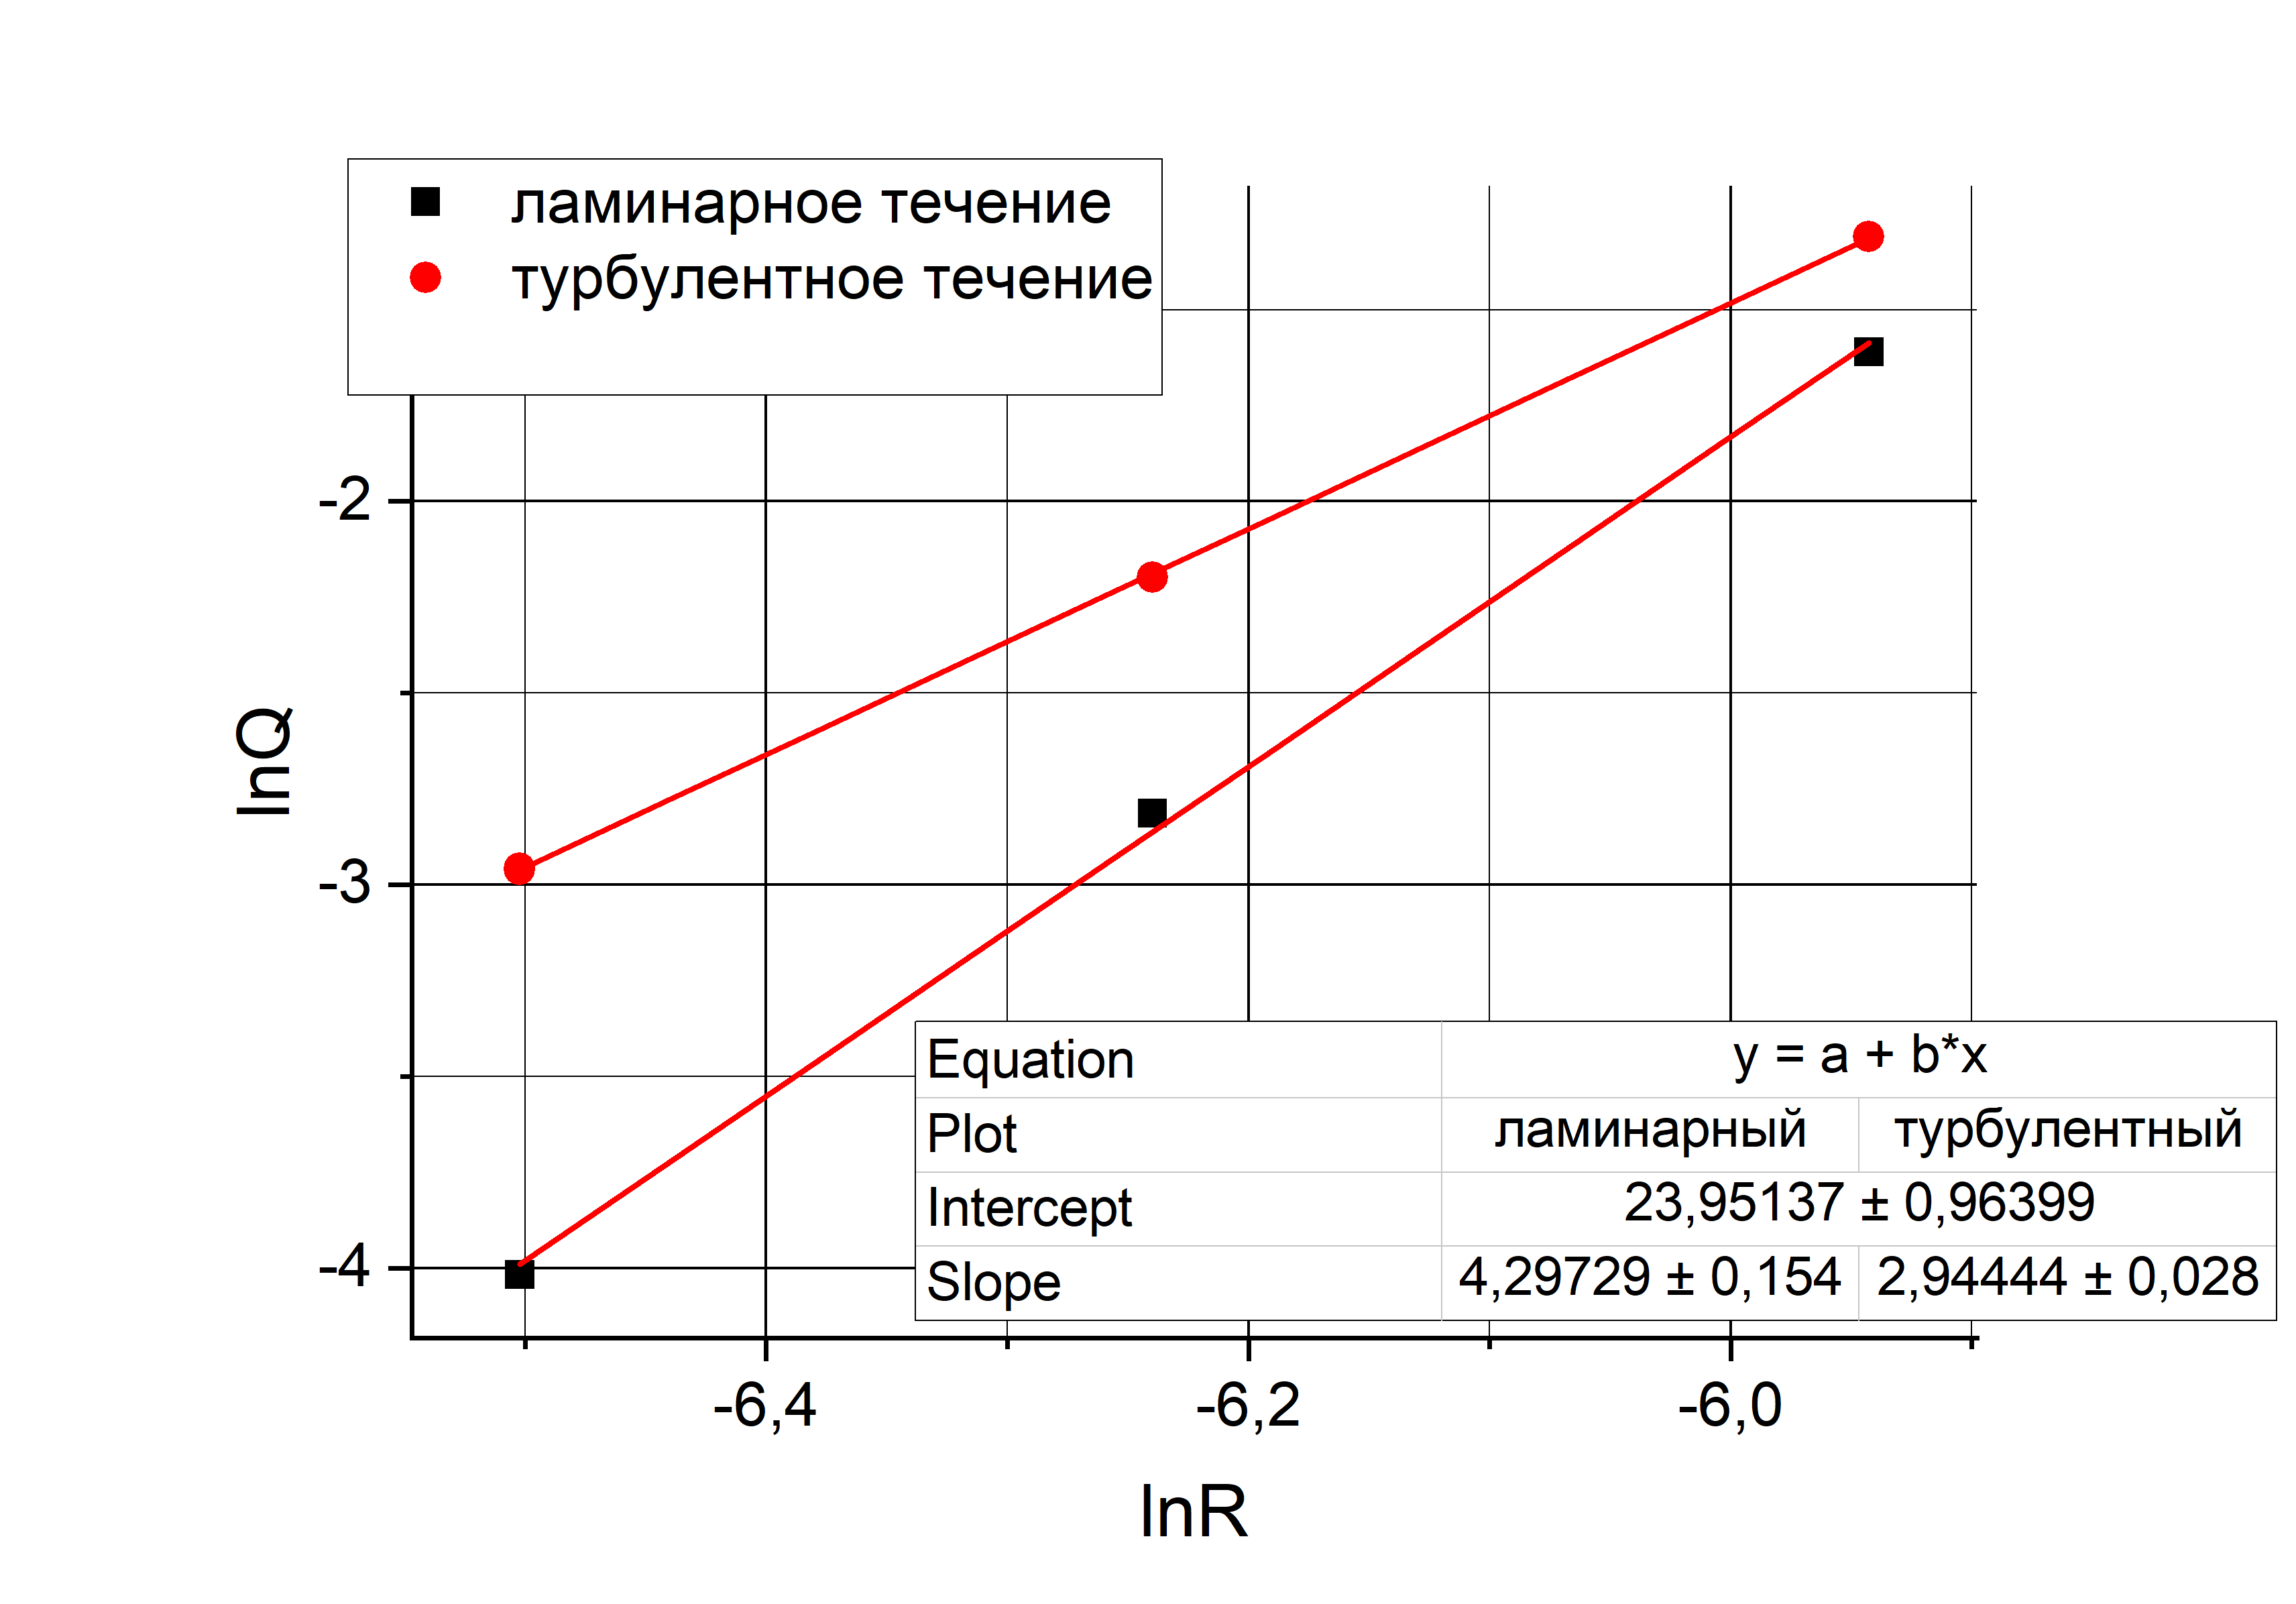
\includegraphics[width=0.8\linewidth]{3}
\caption{Зависимость $lnQ(lnR)$}
\end{figure}

	
\end{document}